\documentclass[journal=jacsat,manuscript=article]{achemso}

\usepackage{epsfig,color,graphicx,amsmath,chemformula,xr}
\usepackage[T1]{fontenc}


\newcommand{\Ang}{\ensuremath{\mathring{\text{A}}}}
\newcommand{\ltwid}{\mathrel{\raise.3ex\hbox{$<$\kern-.75em\lower1ex\hbox{$\sim$}}}}
\newcommand{\gtwid}{\mathrel{\raise.3ex\hbox{$>$\kern-.75em\lower1ex\hbox{$\sim$}}}}
\newcommand{\bra}{\langle}
\newcommand{\ket}{\rangle}
%\newcommand{\sill}{\psi_\mathrm{SILL}}
\newcommand{\sill}{\psi}
\newcommand{\trace}{{\rm Tr}}
\newcommand{\ntilde}{\tilde{n}}
\newcommand{\stilde}{\tilde{s}}
\newcommand{\atilde}{\tilde{\alpha}}
\newcommand{\new}{\color{red}}
\newcommand{\blue}{\color{blue}}
\newcommand{\old}{\color{black}}
\newcommand{\bea}{\begin{eqnarray}}
\newcommand{\eea}{\end{eqnarray}}
%\newcommand{\bea}{\begin{equation} \begin{split}}
%\newcommand{\eea}{\end{split} \end{equation}}
\def\nn{\nonumber\\}


\externaldocument{covalency_main}

\title{
Supplementary Information: \\
Contribution of the covalent component of the hydrogen-bond network to the properties of liquid water
}

\author{Yifei Shi}
\affiliation{Department of Chemistry, McGill University, 801 Sherbrooke St. West, Montreal, QC H3A 0B8, Canada}
\author{Hayden Scheiber}
\affiliation{Department of Chemistry, University of British Columbia, 2036 Main Mall, Vancouver, BC V6T 1Z1, Canada}
\author{Rustam Z. Khaliullin}
\email{rustam.khaliullin@mcgill.ca}
\affiliation{Department of Chemistry, McGill University, 801 Sherbrooke St. West, Montreal, QC H3A 0B8, Canada}


%\date{\today}

\begin{document}


\maketitle
%\clearpage
%\widetext
\setcounter{figure}{0}
%\setcounter{page}{1}
\renewcommand{\thefigure}{S\arabic{figure}}
\renewcommand{\thepage}{S\arabic{page}}
\section{Calculation of the angular distribution function} 

The distribution of HB angles ($\phi \equiv O_{\text{ref}} \cdots O-H$) includes only hydrogen atoms within distance $R$ from the reference oxygen atom and was normalized to account for the $\phi$-dependent volume. While this normalization is different from the one commonly used in the literature, it correctly emphasizes the energetic preference for linear HBs.
%
\bea
g_R(\phi) = \frac{n_R(\phi)}{V_R(\phi) N_R}
\eea
%
where $n_R(\phi)$ is the number of HB angles in the bin between $\phi$ and $\phi + \Delta$, $V_R(\phi)$ is the physical volume of this bin
%
\bea
V_R(\phi) &= \int_0^{2 \pi} d\Theta \int_{\phi}^{\phi+\Delta} \sin \phi\, d\phi \int_0^R r^2 dr = \nn
&= \frac{2 \pi R^3}{3} \left[ \cos (\phi) -\cos (\phi+\Delta) \right] = \nn
&= \frac{2 \pi R^3}{3} \left[ \Delta \sin (\phi) + \frac{1}{2} \Delta^2 \cos (\phi) + O(\Delta^3)\right] , 
\eea
%
and $N_R$ is the number of HBs in all bins.

\section{Density dependence of the devalent system} 

\begin{figure}
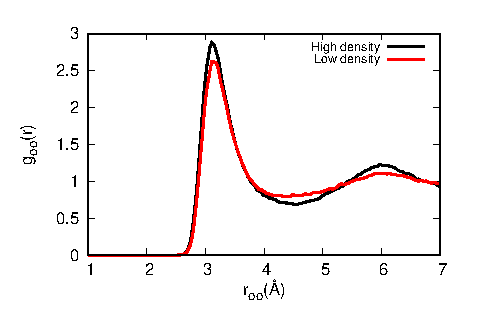
\includegraphics[width=0.45\textwidth]{cp_rdf}
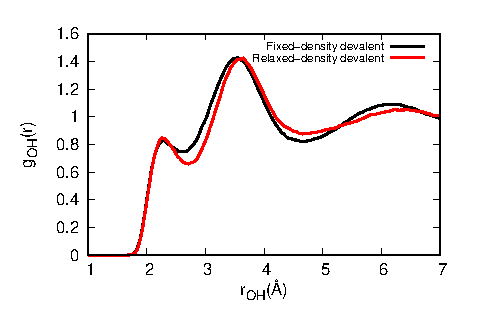
\includegraphics[width=0.45\textwidth]{cp_oh_rdf}
\caption{Oxygen-oxygen and oxygen-hydrogen radial distribution functions for the fixed-density and relaxed-density systems.}\label{Fig:rdf_cp}
\end{figure} 

In order to study the effect of intermolecular covalency on the density of liquid water, NPT-ensemble simulations were performed at 1~atm and 298~K with intermolecular charge transfer switched off. The average density of this system was determined to be 0.85~g$\cdot$cm$^{-3}$. 
This system is denoted the \emph{relaxed-density} devalent system, and contrasted with the \emph{fixed-density} devalent system used throughout the article. 

The oxygen-oxygen and oxygen-hydrogen radial distribution functions for the fixed-density and relaxed-density systems are shown in Figure~\ref{Fig:rdf_cp} for comparison. 
The positions of the peaks do not change significantly and the peaks become less pronounced after density relaxation.

\begin{figure}
%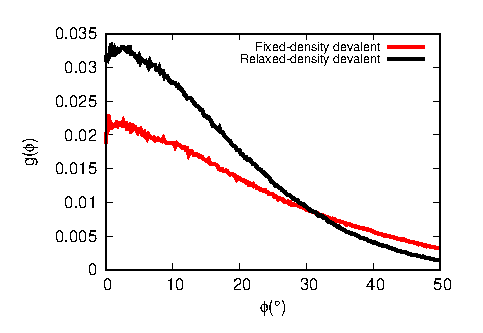
\includegraphics[width=0.45\textwidth]{cp_adf}
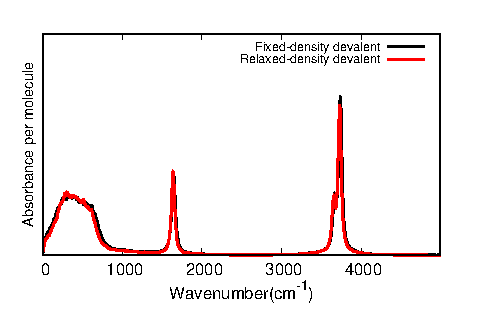
\includegraphics[width=0.45\textwidth]{cp_ir}
\caption{
%Angular distribution function and 
IR spectra for the fixed-density and relaxed-density systems.}\label{Fig:ir_cp}
\end{figure} 

Although the changes in the angular distribution functions are not significant either (Figure~\ref{Fig:ir_cp}), the distribution of HB angles becomes narrower in the relaxed-density system. The IR spectra of the two systems are almost identical (Figure~\ref{Fig:ir_cp}).

%\begin{figure}
%\caption{Angular distribution function for the 2 systems.}\label{Fig:adfcp}
%\end{figure} 
%
%\begin{figure}
%\caption{IR spectrum for the 2 systems.}\label{Fig:ir_cp}
%\end{figure} 

\section{Calculation of the HB lifetime} 

The continuous HB time-correlation function $C_{\text{HB}}(\tau)$ is defined as 
%
\bea
C_{\text{HB}}(\tau) = \frac{\sum_{ij}\langle \theta_{ij}(\tau)\theta_{ij}(0) \rangle}{\sum_{ij}\langle \theta_{ij}(0) \theta_{ij}(0) \rangle} \label{Eq:HBdecay},
\eea
%
where the HB survival function $\theta_{ij}(\tau)$ is equal to 1 if there is a HB formed between molecules $i$ and $j$ \emph{throughout} the time period from $t=0$ to $t=\tau$ and is otherwise equal to zero~\cite{rapaport1983hydrogen,starr1999fast}. 
In the long-time limit, the time-correlation function decays exponentially as shown in Fig~\ref{Fig:HBdecay}. 
The HB lifetime is defined as the rate of its decay $C_{\text{HB}}(\tau) \sim e^{-\tau/\tau_{\text{HB}}}$ and is computed as the slope of the logarithm of $C_{\text{HB}}(\tau)$.


\begin{figure}
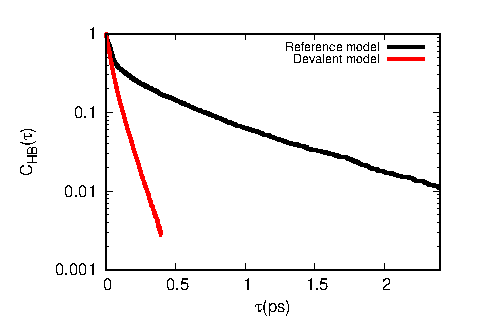
\includegraphics[width=0.4\textwidth]{new_hbdecay}
\caption{HB time autocorrelation function for the reference and devalent systems.} \label{Fig:HBdecay}
\end{figure}

\section{Calculation of the self-diffusion coefficient and shear viscosity} 

\begin{figure}[t]
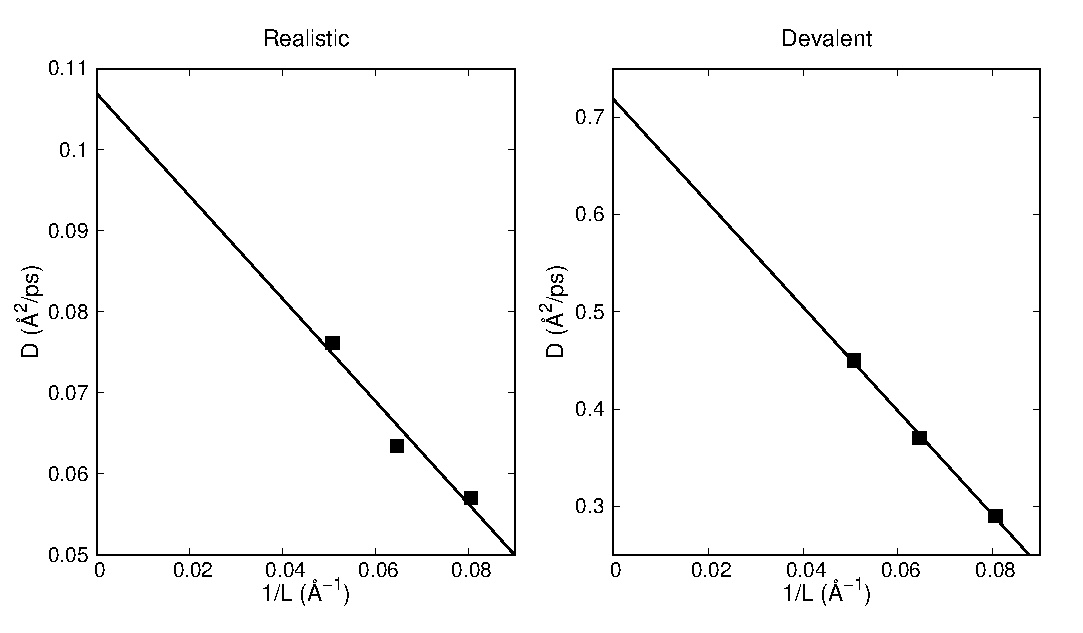
\includegraphics[width=0.47\textwidth]{msd}
\caption{Diffusion constant as a function of the system size, for 64, 125 and 256 water molecules. 
The square dots are from simulation and the solid line is a linear fit.}\label{Fig:dfs}
\end{figure} 

The diffusion constant for a periodic system is known to have strong dependence on the size of the simulation box $L$, due to the long-range drag exerted on a particle by its periodic images~\cite{dunweg1993molecular}. 
Fortunately, the diffusion constant in the infinitely large simulation box $D(\infty)$ can be estimated from several finite-size simulations using the following well-known relation~\cite{dunweg1993molecular}:
%
\bea
D(\infty) = D(L) + \frac{k_BT\zeta}{6\pi \eta L},
\eea
%
where $D(L)$ is the diffusion constant for a system of size $L$, $\eta$ is the translational shear viscosity, and $\zeta$ is a constant of 2.837. 
We calculated the diffusion constant $D(\infty)$ using least squares fitting to the data obtained for systems of 64, 125, and 256 molecules (Figure~\ref{Fig:dfs}). The viscosity is obtained via the slope of the $D(L)$ dependence on $1/L$.

\section{Basis set dependence of the results} 

\begin{figure}
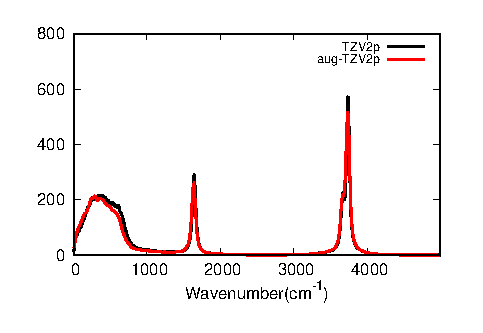
\includegraphics[width=0.45\textwidth]{basis_ir}
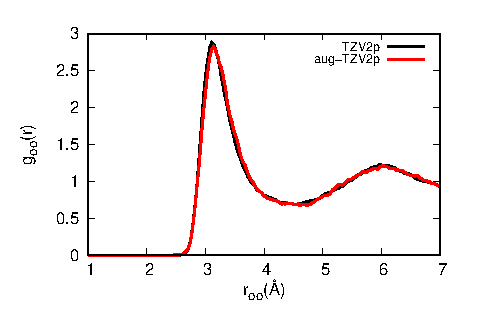
\includegraphics[width=0.45\textwidth]{basis_rdf}
\caption{IR spectra and oxygen-oxygen radial distribution functions calculated with TZV2P and aug-TZV2P basis sets.}\label{Fig:basis}
\end{figure} 

As indicated in the Computational Methods section, the accurate separation of donor-acceptor interactions from polarization effects is verified by performing simulations with two Gaussian basis sets of different sizes. 
To make the test stringent, the TZV2P basis set was extended by adding a set of diffuse functions with small exponents. 
The results of both simulations shown in Figure~\ref{Fig:basis} are practically identical. 
This indicates that TZV2P results are sufficiently stable with respect to a moderate increase in the basis set size. 
For larger basis sets, the role of intermolecular covalency will be spuriously decreased.

\bibliography{covalency}


\end{document}
